\chapter{PROJECT GANTT CHART}
\label{app:gantt}
% TODO: Check the months of activities 1-5 against Table 3.3 of the interim report.
The timeline of the project across Final Year Project~I and~II is shown in Figure~\ref{fig:gantt}. The robustness checks were added in November 2026, after the date-only timestamps had been identified, and are shown as a separate activity.

\begin{figure}[htbp]
\centering
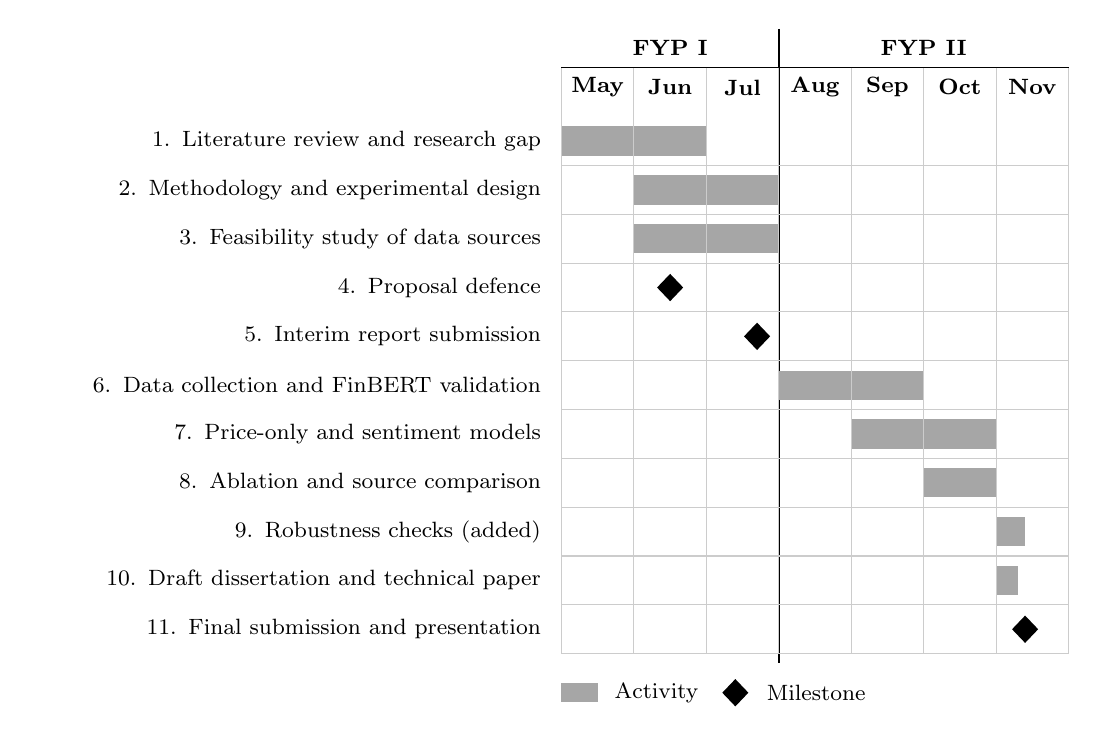
\begin{tikzpicture}[x=0.92cm,y=0.62cm,font=\footnotesize]
  % Columns: May (0) to Nov (6)
  \foreach \m [count=\i from 0] in {May,Jun,Jul,Aug,Sep,Oct,Nov}
    \node[font=\footnotesize\bfseries] at (\i+0.5,0.6) {\m};
  \node[font=\footnotesize\bfseries] at (1.5,1.4) {FYP I};
  \node[font=\footnotesize\bfseries] at (5.0,1.4) {FYP II};
  \draw (0,1.0) -- (7,1.0);
  \draw[thick] (3,1.8) -- (3,-11.2);
  % Rows: label, start month, end month (exclusive), milestone flag
  \foreach \lab/\s/\e/\ms [count=\r from 1] in {
      {1. Literature review and research gap}/0/2/0,
      {2. Methodology and experimental design}/1/3/0,
      {3. Feasibility study of data sources}/1/3/0,
      {4. Proposal defence}/1.5/1.5/1,
      {5. Interim report submission}/2.7/2.7/1,
      {6. Data collection and FinBERT validation}/3/5/0,
      {7. Price-only and sentiment models}/4/6/0,
      {8. Ablation and source comparison}/5/6/0,
      {9. Robustness checks (added)}/6/6.4/0,
      {10. Draft dissertation and technical paper}/6/6.3/0,
      {11. Final submission and presentation}/6.4/6.4/1} {
    \node[anchor=east,align=right,text width=6.4cm] at (-0.15,-\r+0.5) {\lab};
    \draw[gray!40] (0,-\r) -- (7,-\r);
    \ifnum\ms=1
      \fill[black] (\s,-\r+0.5) +(0,0.28) -- +(0.18,0) -- +(0,-0.28) -- +(-0.18,0) -- cycle;
    \else
      \fill[gray!70] (\s,-\r+0.2) rectangle (\e,-\r+0.8);
    \fi
  }
  \foreach \i in {0,...,7} \draw[gray!40] (\i,1.0) -- (\i,-11);
  % Legend
  \fill[gray!70] (0,-12.0) rectangle (0.5,-11.6);
  \node[anchor=west] at (0.6,-11.8) {Activity};
  \fill[black] (2.4,-11.8) +(0,0.28) -- +(0.18,0) -- +(0,-0.28) -- +(-0.18,0) -- cycle;
  \node[anchor=west] at (2.7,-11.8) {Milestone};
\end{tikzpicture}
\caption{Project Gantt Chart, May to November 2026}
\label{fig:gantt}
\end{figure}

\chapter{SOURCE CODE SAMPLE}
\label{app:code}
The full source code is available on GitHub:

{\small\url{https://github.com/AdhamAlwee/Semantic-Analayzer-for-US-Market}}

The functions below, from \texttt{src/ablation.py} and \texttt{src/lag\_robustness.py}, implement the walk-forward splits, the movement labels, the paired block bootstrap and the one-day lag.

\begin{lstlisting}[language=Python,showstringspaces=false,columns=fullflexible,basicstyle=\ttfamily\fontsize{8}{9.5}\selectfont]
def label_movement(returns, band):
    """0 = down, 1 = stable, 2 = up."""
    return np.where(returns > band, 2, np.where(returns < -band, 0, 1))


def walk_forward_splits(dates, horizon, test_years=TEST_YEARS):
    """(test_year, train_idx, test_idx); drops the last `horizon` training rows (purge)."""
    years = dates.dt.year.values
    splits = []
    for year in test_years:
        train_idx = np.where(years < year)[0]
        train_idx = train_idx[:-horizon] if horizon > 0 else train_idx
        test_idx = np.where(years == year)[0]
        if len(train_idx) and len(test_idx):
            splits.append((year, train_idx, test_idx))
    return splits


def block_bootstrap_delta(y_true, pred_base, pred_new, metric,
                          block=10, n_samples=2000, seed=42):
    """Paired moving-block bootstrap of metric(new) - metric(base) on the same test days."""
    rng = np.random.default_rng(seed)
    n = len(y_true)
    n_blocks = int(np.ceil(n / block))
    deltas = np.empty(n_samples)
    for i in range(n_samples):
        starts = rng.integers(0, n - block + 1, size=n_blocks)
        idx = (starts[:, None] + np.arange(block)).ravel()[:n]
        deltas[i] = metric(y_true[idx], pred_new[idx]) - metric(y_true[idx], pred_base[idx])
    observed = metric(y_true, pred_new) - metric(y_true, pred_base)
    p_two_sided = 2 * min(np.mean(deltas <= 0), np.mean(deltas >= 0))
    return {"delta": observed,
            "ci_low": float(np.percentile(deltas, 2.5)),
            "ci_high": float(np.percentile(deltas, 97.5)),
            "p_value": float(min(1.0, p_two_sided))}


def lag_sentiment(df, days=1):
    """One ticker, sorted by date: sentiment features come from `days` trading days earlier."""
    out = df.copy()
    columns = SENTIMENT_FEATURES + COMPANY_SENTIMENT_FEATURES
    out[columns] = out[columns].shift(days).fillna(0)
    return out
\end{lstlisting}
